%!TEX root = ../../report.tex

\subsection{Predicting with Markov model}

A use for the dynamic information of a cell is to improve the prediction of the occupancy of a cell. The prediction mechanism used with PMAC is based on an estimated occupancy value. This value is determined through the update-predict method described in section \vref{sec:cost_interpretation_path_planning}. 
In order to demonstrate the prediction, it has been used on the obstacles. The predict error score is calculated by equation \ref{eq:predict_error_score}. This is calculated for a region of interest around the obstacle position. The number of cells used in the calculation is the number of cell in the region for which the new observation has information. 

\begin{equation}
	Error_{score} = \frac{\sum\limits_{i=1}^{n_{cells}} (p_{predict}(i)-p_{observation}(i))^2}{n_{cells}}
	\label{eq:predict_error_score}
\end{equation} 

In the test only one in every 5 observations were used in the update of the current estimate in order to allow the prediction to engage. All observations were, however, used in the learning of Markov parameters. Figure \ref{fig:markov_predict_obst_2} shows the resulting score for PMAC and a simple previous prediction. The previous predictor uses the last observation as predictor, with the same one in five observations added. The score values are rather small due to the fact that the region of interest also contains static free cells which neither predictor has any trouble with. As PMAC is not initialized with any information on the dynamics these are learned through the observations. 
It is seen that the PMAC predictor does a better job at predicting the occupancy state for this obstacle. The effect of using the PMAC will vary for different obstacles. For the obstacles with low transition probabilities using the previous observation as predictor can be a good approximation and can outperform PMAC, especially if PMAC has not learned  accurate Markov parameters.  

\begin{figure}[htbp]
	\centering
	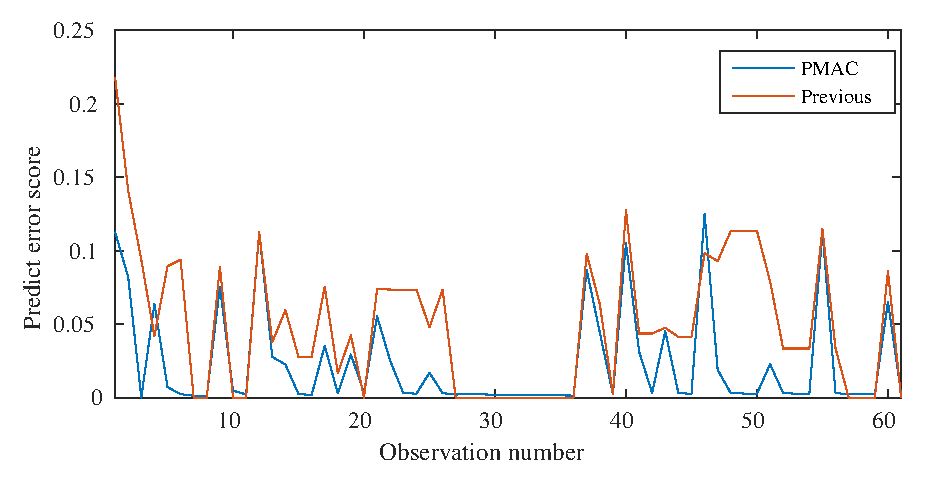
\includegraphics[scale=1]{chapters/evaluation/figures/markov_predict_figs/obstacle2_low.eps}
	\caption{Predict error score for obstacle number 2}
	\label{fig:markov_predict_obst_2}
	
\end{figure}